\documentclass{beamer}
\usepackage[utf8]{inputenc}
\usepackage[spanish]{babel}
\usepackage{graphics}
\usepackage{graphicx}
\usetheme[secheader=true]{Madrid}
\useinnertheme{rectangles}
\usepackage{tikz}
\title{Memorias}
\subtitle{Velocidad y Volumen}
\author[msagre]{Miguel A Sagreras}
\date[2015]{}
%\institution[short name]{long name}
\begin{document}

\begin{frame}
\titlepage
\end{frame}

\section{Primeras computadoras}
\subsection{Electromecánicas Analógicas}
\begin{frame}
\frametitle{Torpedo Data Computer}
\begin{center}
\hfill
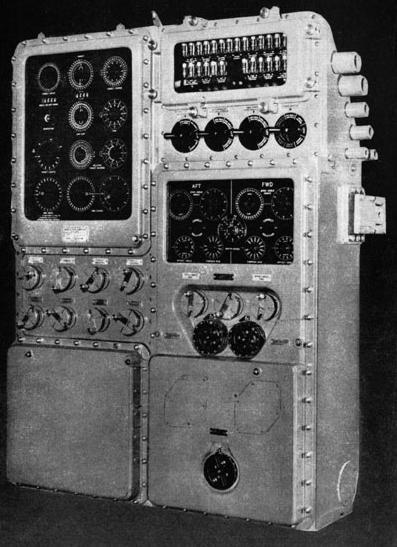
\includegraphics[height=3cm]{TDC-image.jpg}
\hfill
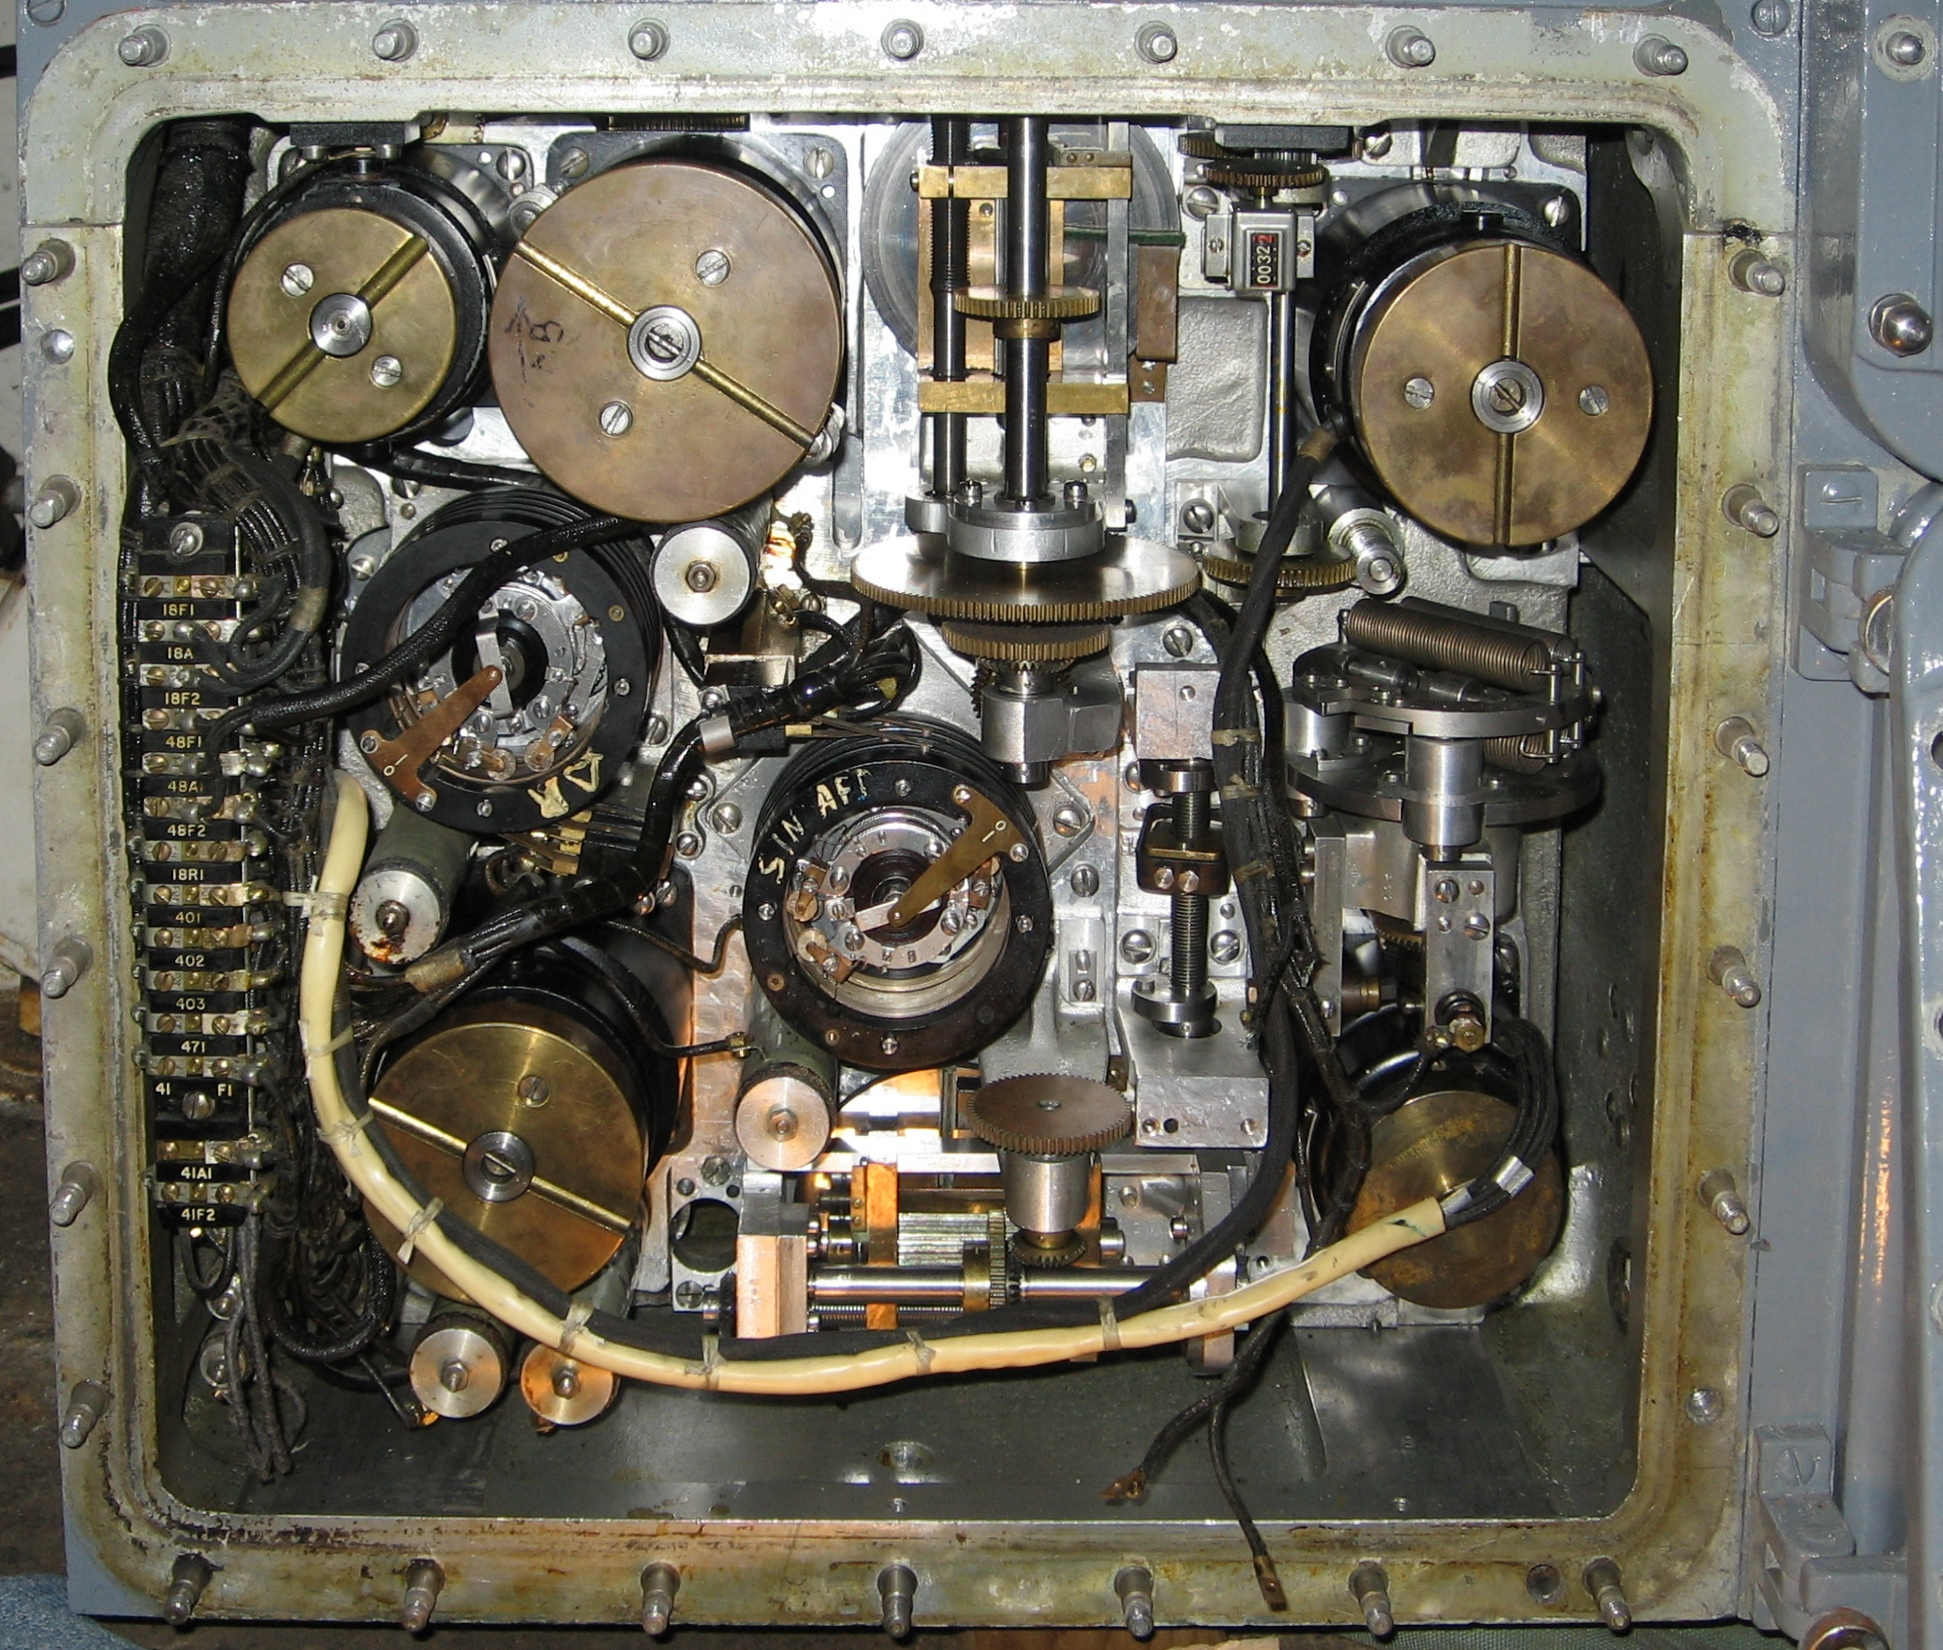
\includegraphics[height=3cm]{TDC-inside.jpg}
\end{center}
\end{frame}

\subsection{Electromecánicas Digitales}
\begin{frame}
\frametitle{Z1}
\begin{center}
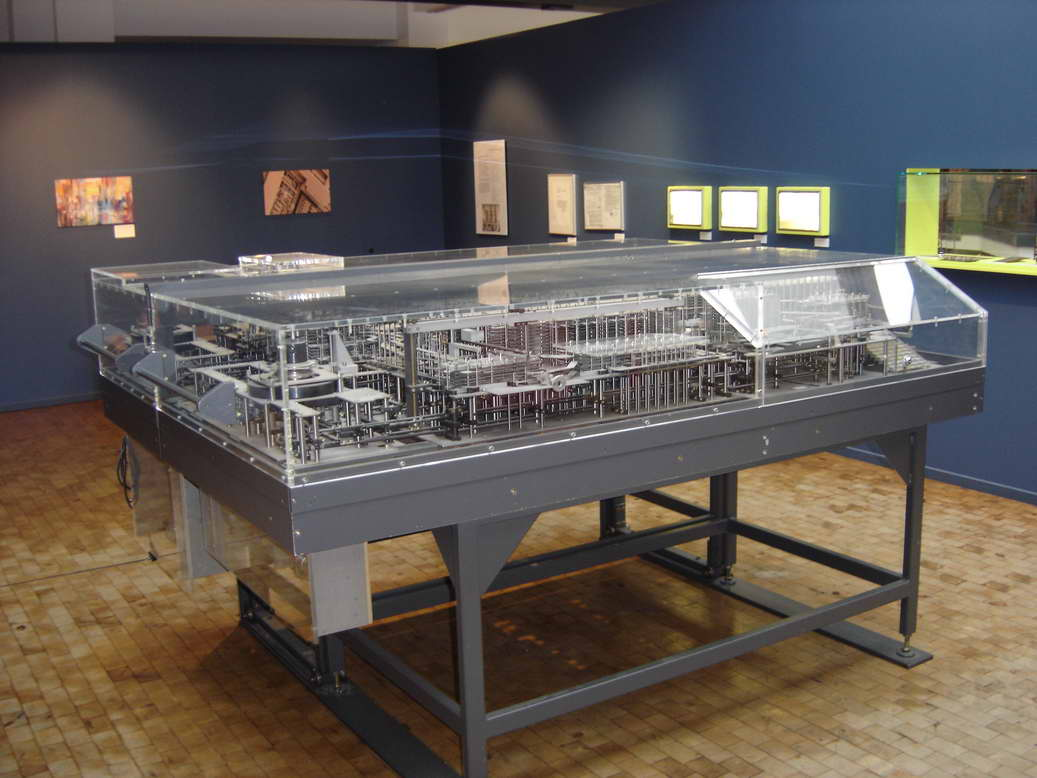
\includegraphics[height=3cm]{Zuse_Z1-2.jpg}
\end{center}
\end{frame}

\subsection{Electromecánicas Digitales}
\begin{frame}
\frametitle{Relays}
\begin{center}
\hfill
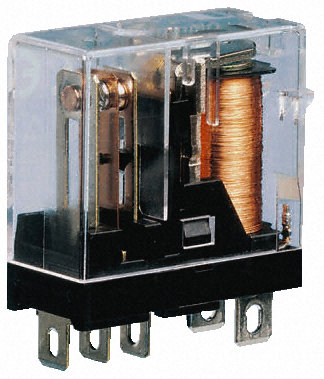
\includegraphics[height=3cm]{relay-imagen.jpg}
\hfill
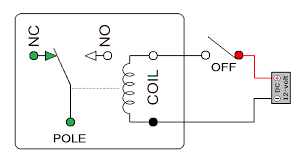
\includegraphics[height=3cm]{relay-diagrama.png}
\end{center}
\end{frame}

\subsection{Electrónicas Digitales}
\begin{frame}
\frametitle{Relays}
\begin{center}
\end{center}
\end{frame}

\section{Memoria}
\begin{frame}
\frametitle{Estructura de la  memoria dinámica}
\begin{figure}[!htb]
\centering
\includegraphics[scale=0.8]{membank.eps}
\end{figure}
\end{frame}

\section{Banco de Memoria}
\begin{frame}
\begin{figure}[!htb]
\centering
\includegraphics[scale=1.0]{chip.eps}
\end{figure}
\end{frame}

\section{Secuencia de acceso}
\begin{frame}
	\begin{itemize}
		\item Acceder a la fila
		\item Acceder a la columna
		\item Recuperar el valor leido
	\end{itemize}
\end{frame}

\section{Timing diagram}
\begin{frame}
\begin{figure}[!htb]
\centering
\includegraphics[scale=1.0]{dram-timings.eps}
\end{figure}
\end{frame}

\section{Timing diagram}
\begin{frame}
\begin{figure}[!htb]
\centering
\includegraphics[scale=1.0]{ddrdram-timings.eps}
\end{figure}
\end{frame}

\section{fpga}
\begin{frame}
\begin{figure}[!htb]
\centering
\includegraphics[scale=1.0]{fpga.eps}
\end{figure}
\end{frame}

\end{document}

